\chapter{Esquemas de aproximação e programação dinâmica}
\label{chap:algs}

Veremos neste capítulo quatro algoritmos de aproximação que utilizam a técnica de programação dinâmica. Estes algoritmos resolvem os problemas da seção \ref{sec:defsProblemas}.

Algo em comum em todos estes algoritmos é o uso da técnica de programação dinâmica. Em todas as soluções que aqui falaremos, a partir da instância original $I$, criaremos uma instância modificada $I'$ aplicando nesta um algoritmo de programação dinâmica para calcular o ótimo para $I'$. 

\begin{figure}
{
\begin{pspicture}(0,-4.24)(15.14,4.24)
\psellipse[linewidth=0.04,dimen=outer](2.99,3.22)(2.79,1.02)
\usefont{T1}{ptm}{m}{n}
\rput(2.8778124,3.81){I}
\psellipse[linewidth=0.04,dimen=outer](2.79,-3.16)(2.79,1.02)
\usefont{T1}{ptm}{m}{n}
\rput(2.7345312,-2.57){I'}
\psline[linewidth=0.04cm,arrowsize=0.05291667cm 2.0,arrowlength=1.4,arrowinset=0.4]{->}(2.72,2.22)(2.66,-2.18)
\psellipse[linewidth=0.04,dimen=outer](12.35,-3.22)(2.79,1.02)
\usefont{T1}{ptm}{m}{n}
\rput(12.444531,-2.67){OPT(I')}
\psellipse[linewidth=0.04,dimen=outer](12.33,3.14)(2.79,1.02)
\usefont{T1}{ptm}{m}{n}
\rput(12.639218,3.49){(1+$\epsilon$) OPT(I)}
\psline[linewidth=0.04cm,arrowsize=0.05291667cm 2.0,arrowlength=1.4,arrowinset=0.4]{->}(5.56,-3.16)(9.56,-3.18)
\psline[linewidth=0.04cm,arrowsize=0.05291667cm 2.0,arrowlength=1.4,arrowinset=0.4]{->}(12.3,-2.24)(12.26,2.16)
\psline[linewidth=0.04cm,linestyle=dotted,dotsep=0.16cm,arrowsize=0.05291667cm 2.0,arrowlength=1.4,arrowinset=0.4]{->}(5.78,3.18)(9.56,3.16)
\usefont{T1}{ptm}{m}{n}
\rput(3.3432813,0.29){Arr(I)}
\usefont{T1}{ptm}{m}{n}
\rput(7.563281,-2.61){A(I')}
\usefont{T1}{ptm}{m}{n}
\rput(13.395156,0.01){T(OPT(I'))}
\end{pspicture} 
}
\caption{Todos os problemas que estudaremos possuem uma característica em comum: As instância original $I$ é alterada para uma instância em $I'$ por um algoritmo que chamamos de $Arr$ (Arredondamento). Em $I'$ aplicamos um algoritmo usando programação dinâmica para achar o caso ótimo. Finalmente, transformamos a solução encontrada em $I'$ para uma solução para I a qual provaremos ser $(1+\epsilon)$ para problemas de minimização e $(1-\epsilon)$ para problemas de maximização.}
\label{fig:esqmaptas}
\end{figure}

A figura \ref{fig:esqmaptas} esquematiza uma representação do que estudaremos nestes quatro problemas levando em conta problemas de minimização. Deixamos a seta que liga a solução para a instância do problema tracejada para demonstrar que o caminho para obtê-la é mediante ao esquema de aproximação.

Todos os esquemas de aproximação que veremos possuem três fases: Transformação da instância original para a instância modificada $I'$ por um algoritmo que chamaramos de $Arr$ (Arredondamento), algoritmo de programação dinâmica para encontrar a solução ótima para $A(I') = OPT(I')$ e transformação da solução $OPT(I')$ para $(1+\epsilon)$. Cada uma das demonstrações que veremos abaixo seguirá estes três passos.

Em todos estes algoritmos, a transformação da solução encontrada para a instância modificada e a instância original é direta. Discutiremos este processo detalhadamente conforme analisarmos cada problema.

Extraímos as demonstrações do livro de Williamson e Shmoys \cite{Williamson}.

\section{O problema da mochila}

\label{ref:ptasMochila}

Vimos na seção \ref{sec:defmochila} a definição para o problema da mochila. Exploraremos uma solução peculiar para o problema, dada pelo algoritmo \ref{alg:pdmochila}.

\begin{algorithm}[H]
\SetAlgoLined
\Entrada{ $I = \{1 \ldots n\}$, vetor de itens. $V = \{v_1, \ldots, v_n\}$, vetor de valores em I  $S = \{s_1, \ldots, s_n\}$, vetor de tamanhos em I; $B$, tamanho da mochila }
$A[1] \leftarrow \{(0,0),(s_1,v_1)\}$ 

\Para{ $j=2$ até $n$}
{
    $A[j] \leftarrow A[j-1] $
    
    \ParaCada{ $(t,w) \in A[j-1]$ }{
    \Se{$t + s_j \leq B $}
    {
        Adicione $(t+s_j,w+v_j)$ em $A[j]$
    }
    
    Remova os pares dominantes de $A[j]$
   }
}

\Retorna{$max_{(t,w) \in A[n]} w $}

\caption{$Mochila$}
\label{alg:pdmochila}
\end{algorithm}

O algoritmo \ref{alg:pdmochila} usa programação dinâmica para resolver o problema da mochila. Ele é baseado nos seguintes passos: Instanciamos um vetor $A[1 \ldots n]$ contendo uma lista de pares $(t,w)$, a qual representa espaço $t \leq B$ e possui valor $w$. Ou seja, existe um conjunto $ S \subseteq \{ 1, \ldots, \}$ tal que $\sum_{i \in S} s_i = t \leq B$ e $\sum_{i \in S} v_i = w$. Cada elemento do vetor $A$ é outro vetor $A[j]$, o qual não contém todos os pares possíveis até o elemento $j$, apenas os mais eficientes. Para fazer isto, introduzimos o conceito de pares dominantes.

Para um par $(t,w)$ pertencente a $A[j]$, com $ 1 \leq j \leq n$, dizemos que este domina outro par $(t',w')$ pertencente à $A[j]$ se $t \leq t'$ e $w \geq w'$. Ou seja, $(t,w)$ ocupa igual ou menos espaço e valor no mínimo igual. Para $A[j]$ removeremos os pares dominados, ou seja, manteremos aqueles os quais esta propriedade não se aplique para todos os elementos de $A[j]$.

Dizemos que o vetor representado por $A[j]$ contém apenas pares dominantes, e assume a forma $(t_1,w_1), \ldots, (t_k,w_k)$, com $t_1 < t_2 < \ldots < t_k$ e $w_1 < w_2 < \ldots < w_k$. Ou seja, o vetor $A[j]$ é ordenado em ordem crescente de peso.

Definimos $V$ como a soma de todos os valores dos itens de uma instância do problema $V= \sum_{i=1}^{n} v_i$. Então $V$ é o maior valor possível para o problema, e $A[j]$ pode conter no máximo $V+1$ pares na lista (Incluímos também o par $(0,0)$, pois assumimos na definição que os pesos e tamanhos são inteiros (A ideia de pares dominantes assegura um único par contendo o mesmo peso na lista). Pelo mesmo raciocínio, não podem existir mais de $B+1$ pares em $A[j]$.

O algoritmo \ref{alg:pdmochila} executa os seguintes passos: Instancia o vetor $A[j]$, sendo seu primeiro elemento $A[1] \leftarrow \{(0,0),(s_1,v_1)\}$. A partir do segundo elemento até $n$, o algoritmo atribui $A[j] \leftarrow A[j-1]$ e para cada par $(t,w)$ em $A[j]$ inclui um novo par $(t+s_j,w+v_j)$ se $t+s_j \leq B$. Finalmente o algoritmo remove os pares dominantes da lista.

A remoção dos pares dominantes pode ser feita em tempo na ordem do tamanho da lista. Mostraremos a partir do lema abaixo.

\begin{lema}[Remoção dos pares dominantes]
\label{lem:remparesdom}
A remoção dos pares dominantes pode ser executada em tempo $O(\min\{V,B\})$.
\end{lema}

\begin{proof}
Suponha que estamos no início da linha 9 do algoritmo, e que $A[j]$ esteja ordenada pelo índice $t$ e contenha ainda os pares dominantes e dominados. Mostraremos que basta percorrer um número $O(\abs{A[j]}) = O(\min\{V,B\})$ para remover todos os pares dominados. Suponha dois pares $(t,w)$ e $(t',w')$ de forma que $(t,w)$ domina $(t',w')$.
Precisamos avaliar dois casos, onde $t=t'$ e $t \neq t'$. No primeiro caso, sabemos que $w \leq w'$ e além disso $t$ e $t'$ são adjacentes em $A[j]$. Logo percorrendo a lista uma vez e comparando os pares adjacentes é suficiente para remover $(t',w')$. Caso exista $(t'',w'')$ dominado por $(t,w)$ de forma que $t=t'=t''$ basta "travar" a execução em $t$ após $t'$ ser removido e repetir a remoção, sem aumentar a ordem de execução do algoritmo.
Resta-nos mostrar casos onde $t' > t$. Se $t'$ for adjacente a $t$ na ordem de execução aplica-se o mesmo procedimento descrito para $t=t'$. Caso contrário, se $t'$ não é adajcente a $t$, então existe um par $(\hat{t}, \hat{w})$, tal que $t < \hat{t} \leq t'$ tal que não há relação de dominância entre $(\hat{t}, \hat{w})$ e $(t,w)$. Neste caso sabemos que $\hat{w} > w \leq w'$ e $\hat{t} \leq t'$. Logo $(\hat{t}, \hat{w})$ domina $(t',w')$ e ambos são adjacentes. 

Finalmente, para manter o vetor contido em $A[j]$ ordenado, basta formar duas listas, uma contendo $A[j-1]$ e outra contendo os elementos formados da adição de $(s_j,v_j)$ em $A[j-1]$ e intercalá-las, o que pode-se ser feito na ordem de $A[j]$ operações.

Logo o custo para ordenar e eliminar os pares dominados é de $O(\abs{A[j]}) = O(\min\{V,B\})$ de instruções, esta última equação sendo válida porque é impossível termos um número de itens maior a $V+1$ ou $B+1$ pares.
\end{proof}

Afirmamos que o algoritmo \ref{alg:pdmochila} encontra a solução ótima para o problema da mochila, através do teorema abaixo.

\begin{teorema}
O algoritmo \ref{alg:pdmochila} calcula a solução ótima para o problema da mochila.
\end{teorema}

\begin{proof}
Provamos por indução que em $j$, $A[j]$ contém somente (e todos) os pares dominantes para todos os estados até $j$. O caso base $A[1] \leftarrow \{(0,0),(s_1,v_1)\}$ é válido. Agora suponha que seja válido para $A[j-1]$. Sendo $S \subseteq \{1, \ldots, j\}$, e $t=\sum_{i \in S} s_i \leq B$ e $w = \sum_{i \in S} v_i$. Afirmamos que existe um par $(t',w') \in A[j]$ que domina o par $(t,w)$.

Avaliaremos em dois casos, no primeiro $j \neq S$. Neste caso, $A[j]$ conterá apenas $(t',w')$, pois $(t,j)$ é obtido de $A[j-1]$ mas removido na linha 9 do algoritmo \ref{alg:pdmochila}.

No segundo caso $j \in S$. Definimos $S' = S - {j}$, o qual por hipótese de indução, há algum $(\hat{t},\hat{w}) \in A[j-1]$ que domina ($\left(\sum_{i \in S'} s_i,\sum_{i \in S'} v_i\right)$), então $\hat{t} \leq \sum{i \in S'} s_i$ e $\hat{w} \geq \sum_{i \in S'} v_i$. Então o algoritmo adicionará o par $\left(\hat{t} + s_j, \hat{w} + v_j \right)$ para $A[j]$, pois $\hat{t} + s_j \leq t \leq B$ e $\hat{w} + v_j \geq w$. Assim, se um par $(t',w')$ domina um par $(t,w)$ em $j-1$, este continuará dominando em $j$ e a remoção de pares dominados em $j-1$ não afeta a solução ótima.

\end{proof}

A partir do \ref{alg:pdmochila} vemos que o algoritmo consome tempo $O(n \min\{V,B\})$, pois gasta $n$ passos para formar o vetor $A$ e mais $O(n \min\{V,B\})$ para eliminar os passos dominados.

O algoritmo \ref{alg:pdmochila} não é um algoritmo polinomial. Rotineiramente codificamos o tamanho da mochila em base binária. Dobrar o tamanho da mochila neste caso aumenta em $\log_2 2 = 1$ o tamanho da instância, enquanto o número de passos na remoção de pares dominantes aumenta $O(B) = 2$. Aumentando em $2^{10}$ o valor da entrada aumentamos em $10$ seu tamanho e em $1024$ o número de passos executados para eliminar os pares dominantes.

Entretanto, se a entrada do algoritmo \ref{alg:pdmochila} for codificada em unário, ele executa em tempo polinomial em relação ao seu tamanho. Dizemos que este é então um algoritmo \textit{pseudo-polinomial} \cite{Williamson}.

Apresentamos uma maneira de obter uma $(1 - \epsilon)$-aproximação para o problema da mochila a partir de arredondamento utilizando o algoritmo \ref{alg:pdmochila}.

Para fazê-lo, iremos arredondar a instância em inteiros múltiplos de uma grandeza que chamaremos de $\mu$ e converter cada valor $v_i$ para o múltiplo mais próximo de $\mu$. Mais precisamente, definimos uma instância modificada $I'$, onde os valores dos itens não são mais $v_i,\ldots,v_n$, mas $v_i',\ldots,v_n'$ e $v_i' = \lfloor v_i / \mu \rfloor$, para cada item $i$. Executamos então o algoritmo \ref{alg:pdmochila} usando $I'$. Mostraremos que se fizermos esta alteração poderemos calcular a aproximação em tempo polinomial.

Esta alteração para $\mu$ não provoca alterações muito grandes no problema original e que além disso, conseguiremos executar o algoritmo em tempo polinomial. Faremos primeiro uma estimativa: Se usarmos valores $\tilde{v_i} = v_i'\mu$ ao invés de $v_i$, a imprecisão em cada valor $v_i$ seria de no máximo $\mu$, logo cada solução factível sofreria uma mudança de no máximo $\mu$ unidades.

Desejamos que o erro seja de no máximo $\epsilon$ vezes o limitante inferior da solução do problema, o qual é o valor do maior item da mochila (A solução mais simples consiste em escolher o item de maior valor). Sendo assim, definimos $M$ como sendo o tamanho do item de maior valor:

\begin{equation} 
M = \max_{i \in I} v_i
\end{equation}

Assim, se fizermos o erro $n\mu$ da solução igual ao erro do limitante inferior, teremos:

\begin{equation}
n\mu = \epsilon M
\end{equation}

E para gerar $I'$ dividiremos cada valor $v_i$ por $\mu$, com $\mu$ sendo:

\begin{equation}
\mu = \epsilon M / n
\end{equation}

Com os valores divididos por $\mu$, o vetor de valores $V' = \sum_{i=1}^{n} v_i'$ fica sendo:

\begin{equation}
V' = \sum_{i=1}^{n} v_i' = \sum_{i=1}^n \left\lfloor \frac{v_i}{\epsilon M / n} \right\rfloor
\end{equation}

O último termo desta soma é na verdade, uma soma de progressão aritmética dividida por um fator $\epsilon$. Esta soma tem uma característica de seu resultado ser $O(n^2)$. Sabemos então que $V' = O(n^2/ \epsilon)$. Observando a ordem do algoritmo \ref{alg:pdmochila}, se executarmos este algoritmo com esta aproximação, o tempo de execução será de:

\begin{equation}
O(n \min\{V,B\}) = O(n^3/ \epsilon)
\end{equation}

Logo o arredondamento proporcionou executar o algoritmo em tempo polinomial.

O algoritmo \ref{alg:pdmochilaptas} converte a instância $I$ em $I'$ e calcula a $(1 - \epsilon)$ aproximação. 

\begin{algorithm}[H]
\SetAlgoLined
\Entrada{ $I = \{1 \ldots n\}$, vetor de itens. $V = \{v_1, \ldots, v_n\}$, vetor de valores em I  $S = \{s_1, \ldots, s_n\}$, vetor de tamanhos em I }

$M \leftarrow \max_{i \in I} v_i$ 

$\mu \leftarrow \epsilon M/n$ 

$v_i' \leftarrow \lfloor v_i/ \mu \rfloor$ para todo $i \in I$

Execute o algoritmo \ref{alg:pdmochila} para a instância do problema da mochila com valores $v_i'$.

\caption{AproximaçãoMochila}
\label{alg:pdmochilaptas}
\end{algorithm}

Finalmente nos resta mostrar que o algoritmo \ref{alg:pdmochilaptas} calcula uma $(1-\epsilon)$-aproximação para o problema da mochila.

\begin{teorema}
O algoritmo \ref{alg:pdmochilaptas} é um esquema de aproximação polinomial para o problema da mochila
\end{teorema}

\begin{proof}

Precisamos mostrar que o algoritmo retorna uma solução cujo valor é pelo menos $(1 - \epsilon)$ a solução ótima. Seja $S$ o conjunto de itens retornados pelo algoritmo e $O$ o conjunto de itens da solução ótima. Sabemos que $M \leq OPT$, ou seja, pois qualquer solução envolve escolher um ou mais itens (Neste caso estamos escolhendo o mais valioso). Além disso, pela definição de $v_i'$, $\mu v_i' \leq v_i \leq \mu (v_i'+1)$, além de $\mu v_i' \geq v_i - \mu$. Aplicando as definições de arredondamento, além de que $S$ é a solução ótima para a instância modificada $I'$, chegamos nas equações abaixo:

\begin{align*}
\sum_{i \in S} v_i &\geq \mu \sum_{i \in S}{} v_i'  \\
&\geq \mu \sum_{i \in O} v_i'  \\
&\geq  \sum_{i \in O} v_i - \abs{O} \mu  \\
&\geq \sum_{i \in O} v_i - n \mu  \\
&= \sum_{i \in O} v_i - \epsilon M  \\
&\geq OPT - \epsilon OPT = (1 - \epsilon) OPT
\end{align*}

\end{proof}

\section{Escalonamento de tarefas em máquinas paralelas idênticas}
\label{sec:escalonamento}

Achamos conveniente falar do problema em duas partes. Na primeira, apresentaremos duas $\alpha$-aproximações (Seção \ref{sec:escalonamentocte}). Em seguida, falamos de um esquema de aproximação combinado a programação dinâmica para resolvê-lo (Seção \ref{sec:escalonamentoptas}).

Falamos brevemente das definições que usaremos no restante desta seção. Temos como entrada para o problema $n$ tarefas e $m$ máquinas idênticas. Cada tarefa $j = 1, \ldots, n$ executa em tempo $p_j$ em apenas uma máquina sem interrupção. Cada máquina executa apenas uma tarefa por vez. 

O objetivo é completar todas as tarefas o mais rápido possível. Definiremos como $c_j$ o tempo no qual a tarefa termina (Presumindo que o escalonamento inicia-se no tempo 0). Queremos então encontrar $c_{\max} = \max_{j = 1, \ldots, n} c_j$, o qual chamaremos de \textit{largura} do escalonamento de tarefas.

Para uma dada instância I do problema, a solução ótima, a qual rotineiramente chamamos de $OPT(I)$ será neste problema conhecida como $c_{\max}^*$.

\subsection{Duas $\alpha$-aproximações para o problema}
\label{sec:escalonamentocte}

Veremos dois algoritmos de aproximação apresentados no livro de Williamson \cite{Williamson}.

O primeiro é conhecido como algoritmo de busca local.

\begin{algorithm}[H]
\SetAlgoLined
\Entrada{ $J$ = $\{1, \ldots, n\}$, vetor de tarefas. $M$ = $\{1, \ldots, n\}$, vetor de máquinas e P = $\{p_1, \ldots, p_n \}$, vetor de tempos de processamento de cada tarefa }

Defina $ME \leftarrow Matriz_{M \times J}$

Inicie $ME$ com qualquer sequência aleatória de tarefas por máquina

\Enqto{ $mv \leftarrow MaquinaVazia(ME,c_l-p_l)$} { TrocaTarefa($ME$, $l$, $mv$)  }

\caption{Busca Local}
\label{alg:buscalocalescalonamento}
\end{algorithm}

O algoritmo \ref{alg:buscalocalescalonamento} apresenta o pseudocódigo para este algoritmo de busca local. O princípio do mesmo é instanciar uma matriz de máquinas por tarefas, um escalonamento qualquer e depois, verificar se para a última tarefa há alguma máquina a qual pode completá-la antes (Basta verificar se a máquina está disponível para processar tarefas em tempo $c_l - p_l$) e então transferir a última tarefa a completar para esta máquina.

A figura \ref{fig:buscalocalescalonamento} exemplifica uma execução do algoritmo.

\begin{figure}
\centering
\scalebox{1} % Change this value to rescale the drawing.
{
\begin{pspicture}(0,-4.6025)(7.2825,4.565)
\definecolor{color137b}{rgb}{0.6705882352941176,0.6627450980392157,0.6862745098039216}
\definecolor{color313b}{rgb}{0.996078431372549,0.996078431372549,0.996078431372549}
\usefont{T1}{ptm}{m}{n}
\rput(0.060625,4.3725){1}
\usefont{T1}{ptm}{m}{n}
\rput(0.0659375,3.9725){2}
\usefont{T1}{ptm}{m}{n}
\rput(0.06890625,3.5725){3}
\usefont{T1}{ptm}{m}{n}
\rput(0.078125,3.1725){4}
\usefont{T1}{ptm}{m}{n}
\rput(0.06734375,2.7725){5}
\usefont{T1}{ptm}{m}{n}
\rput(0.060625,1.9725){1}
\usefont{T1}{ptm}{m}{n}
\rput(0.0659375,1.5725){2}
\usefont{T1}{ptm}{m}{n}
\rput(0.06890625,1.1725){3}
\usefont{T1}{ptm}{m}{n}
\rput(0.078125,0.7725){4}
\usefont{T1}{ptm}{m}{n}
\rput(0.06734375,0.3725){5}
\usefont{T1}{ptm}{m}{n}
\rput(0.060625,-0.4275){1}
\usefont{T1}{ptm}{m}{n}
\rput(0.0659375,-0.8275){2}
\usefont{T1}{ptm}{m}{n}
\rput(0.06890625,-1.2275){3}
\usefont{T1}{ptm}{m}{n}
\rput(0.078125,-1.6275){4}
\usefont{T1}{ptm}{m}{n}
\rput(0.06734375,-2.0275){5}
\psframe[linewidth=0.04,dimen=outer](2.0025,4.5625)(0.3625,4.2225)
\psframe[linewidth=0.04,dimen=outer](4.1425,4.5625)(1.9625,4.2225)
\psframe[linewidth=0.04,dimen=outer](5.7225,4.5625)(4.1225,4.2225)
\psframe[linewidth=0.04,dimen=outer,fillstyle=solid,fillcolor=color137b](7.2825,4.5625)(5.6825,4.2225)
\psframe[linewidth=0.04,dimen=outer,fillstyle=solid](1.9425,1.7625)(0.3425,1.4225)
\psframe[linewidth=0.04,dimen=outer](1.9825,2.2025)(0.3425,1.8625)
\psframe[linewidth=0.04,dimen=outer](4.1225,2.2025)(1.9425,1.8625)
\psframe[linewidth=0.04,dimen=outer,fillstyle=solid,fillcolor=color137b](5.7025,2.2025)(4.1025,1.8625)
\psframe[linewidth=0.04,dimen=outer,fillstyle=solid](1.9225,-0.6575)(0.3225,-0.9975)
\psframe[linewidth=0.04,dimen=outer](1.9625,-0.2375)(0.3225,-0.5775)
\psframe[linewidth=0.04,dimen=outer,fillstyle=solid,fillcolor=color137b](4.0825,-0.2375)(1.9025,-0.5775)
\psframe[linewidth=0.04,dimen=outer,fillstyle=solid,fillcolor=color313b](1.9225,-1.0575)(0.3225,-1.3975)
\usefont{T1}{ptm}{m}{n}
\rput(0.080625,-2.8475){1}
\usefont{T1}{ptm}{m}{n}
\rput(0.0859375,-3.2475){2}
\usefont{T1}{ptm}{m}{n}
\rput(0.08890625,-3.6475){3}
\usefont{T1}{ptm}{m}{n}
\rput(0.098125,-4.0475){4}
\usefont{T1}{ptm}{m}{n}
\rput(0.08734375,-4.4475){5}
\psframe[linewidth=0.04,dimen=outer,fillstyle=solid](1.9425,-3.0775)(0.3425,-3.4175)
\psframe[linewidth=0.04,dimen=outer](1.9825,-2.6575)(0.3425,-2.9975)
\psframe[linewidth=0.04,dimen=outer,fillstyle=solid,fillcolor=color313b](1.9425,-3.4775)(0.3425,-3.8175)
\psframe[linewidth=0.04,dimen=outer](2.5225,-3.8775)(0.3425,-4.2175)
\end{pspicture} 
}
\caption{Exemplo de execução do algoritmo \ref{alg:buscalocalescalonamento} supondo que o algoritmo alocou inicialmente todas as tarefas na primeira máquina.}
\label{fig:buscalocalescalonamento}
\end{figure}

O algoritmo executa $O(n)$ passos (Assumimos que neste caso, $m$ é constante). Vamos agora mostrar que ele é uma 2-aproximação para o problema do escalonamento.

Vamos fornecer alguns limites para o problema. Sabemos que o tempo $c_{max}^{*}$ é no mínimo o tempo da tarefa mais longa, já que todas as tarefas devem ser processadas:

\begin{equation}
\label{equ:escpj}
c_{max}^{*} \geq \max_{j=1,\ldots,n} p_j
\end{equation}

Além disso, precisamos executar $P = \sum_{j=1}^n p_j$ unidades de processamento para completar a execução de tarefas. Em média, uma máquina deve processar então aproximadamente $P/m$ unidades de processamento. Sabemos que se $P$ não for múltiplo do número de máquinas alguma máquina executará um pouco acima da média, de forma que o tempo de execução para o caso ótimo é no mínimo:

\begin{equation}
\label{equ:sumcmax}
c_{max}^{*} \geq \sum_{j=1}^{n} p_j / m
\end{equation}

Para analisar o tempo do algoritmo de busca local, seja $l$ a última tarefa a executar. O horário em que esta tarefa termina é denotado por $c_l$, que é o mesmo que $c_max$, ou tempo objetivo. Sabemos que se o algoritmo terminou com esta tarefa em $c_l$ é porque nenhuma outra máquina estava disponível para completá-la antes. Denotamos por $S_l$ o tempo de início da tarefa $l$, $S_l = C_l - p_l$. Podemos particionar esta execução em dois períodos, de 0 até $S_l$ e $p_l$. Sabemos pela equação \ref{equ:escpj} que $p_l \leq c_{\max}^*$. Quanto ao período antes da última tarefa executar, as máquinas realizaram no máximo $mS_l$ unidades de trabalho, o que não pode ser superior ao total de trabalho a ser feito, caso contrário a tarefa $l$ já teria acabado. Sendo assim:

\begin{equation}
\label{equ:sl}
S_l \leq \sum_{j=1}^{n} p_j / m
\end{equation}

Combinando \ref{equ:sumcmax} com \ref{equ:sl} observamos que $S_l \leq c_{max}^*$. Sendo assim, a largura, ou tempo máximo de execução para este algoritmo é de $2c_{max}^*$.

Encontraremos um resultado ligeiramente melhor no teorema abaixo.

\begin{teorema}
O algoritmo \ref{alg:buscalocalescalonamento} é uma 2-aproximação
\end{teorema}

\begin{proof}

Na verdade, com o mesmo raciocínio da equação \ref{equ:sumcmax} chegamos na verdade a um limite um pouco menor para $S_l$:

\begin{equation}
S_l \leq \sum_{j \neq l} p_j / m
\end{equation}

Já que alguma máquina pode executar além da média e o tempo de $S_l$ ser maior do que a média. E assim o tempo total de execução passa a ser:

\begin{equation}
p_l + \sum_{j \neq l} p_j / m = \left(1 - \frac{1}{m}\right) p_l + \sum_{j=1}^{n} p_j / m
\end{equation}

Aplicando os limites das equações anteriores, chegamos a:

\begin{equation}
p_l + \sum_{j \neq l} p_j / m \leq \left(2-\frac {1}{m}\right)c_{max}^*
\end{equation}

E então melhoramos um pouco nossa $2$-aproximação, cuja melhoria é mais significativa com um número menor de máquinas.

\end{proof}

Apresentaremos agora um algoritmo guloso para resolver o problema. Uma parte deste algoritmo será aproveitada na próxima seção quando falarmos da aproximação que buscamos.

Chamaremos este algoritmo de \textit{escalonamento por listas}. Dada uma lista de tarefas, arbitrariamente ordenada, este algoritmo seleciona a máquina com menor carga e atribui à ela a tarefa no topo da lista e assim sucessivamente. Não apresentaremos o pseudocódigo deste algoritmo.

O teorema abaixo é válido:

\begin{teorema}
O algoritmo de escalonamento por listas é uma 2-aproximação para o problema
\end{teorema} 

\begin{proof}
Dada a saída do algoritmo de escalonamento por listas, fornecemos esta como entrada para o algoritmo de busca local. Este último, ao executar, não alterará a ordem de nenhuma tarefa, pois a última tarefa escalonada pelo algoritmo de listas foi já alocada pela máquina que poderia terminar no tempo mais recente. Sendo assim, a análise que fizemos para a última tarefa $S_l$ também vale e assim chegamos à uma 2-aproximação.
\end{proof}

Na verdade, há um teorema que demonstra que este algoritmo de escalonamento é na verdade uma $4/3$-aproximação para o problema do escalonamento. Não o demonstraremos aqui.

\subsection{Esquema de aproximação polinomial para o problema do escalonamento}
\label{sec:escalonamentoptas}

Veremos nesta seção dois esquemas de aproximação polinomial para o problema do escalonamento. O primeiro deles trata do número de máquinas como constante e o segundo, como entrada do problema.

Começamos com uma variação do problema onde o número $m$ de máquinas é constante. Dado um número de entrada $i$, vamos definir uma família de algoritmos $A_i$ e focar em especial em um algoritmo $A_k$.

Vamos dividir as tarefas em dois grupos: Longas e curtas. Uma tarefa $p_l$ é curta se:

\begin{equation}
p_l \leq \frac{1}{km} \sum_{j=1}^{n} p_j
\end{equation}

Caso contrário $p_l$ é uma tarefa longa. Vale lembrar que o número de tarefas longas é menor que $km$, pois:

\begin{equation}
\label{equ:kmlong}
km p_l > \sum_{j=1}^{n} p_j
\end{equation}

Ou seja, com mais de $km$ tarefas longas teríamos mais trabalho do que fornecido pela instância do problema.

O algoritmo $A_k$ executará da seguinte forma: Dados $k$ e $m$ como constantes, encontraremos, enumerando todos os casos, o escalonamento ótimo para todas as tarefas longas. Depois, aplicaremos o algoritmo de escalonamento por listas nas tarefas curtas.

\begin{algorithm}[H]
\SetAlgoLined
\Entrada{ $J$ = $\{1, \ldots, n\}$, vetor de tarefas. $M$ = $\{1, \ldots, n\}$, vetor de máquinas e P = $\{p_1, \ldots, p_n \}$, vetor de tempos de processamento de cada tarefa }

Defina $ME \leftarrow Matriz_{M \times J}$

Defina $P_{long}$ com todas as tarefas onde $p_l > \sum_{j=1}^{n} p_j / km$

Defina $P_{short}$ com todas as tarefas onde $p_l \leq \sum_{j=1}^{n} p_j / km$

Encontre o escalonamento ótimo para $P_{long}$

Execute o algoritmo \ref{alg:buscalocalescalonamento} com os dados de entrada, matriz $ME$ para $P_short$

\caption{$A_k$}
\label{alg:ak}
\end{algorithm}

O algoritmo \ref{alg:ak} apresenta o pseudocódigo para o algoritmo $A_k$.

No algoritmo de aproximação constante, deduzimos a seguinte inequação para o tempo máximo de execução:

\begin{equation}
\label{equ:shortjob}
c_{max} \leq pl + \sum_{j \neq 1} p_j / m
\end{equation}

Analisamos este algoritmo da mesma maneira que analisamos a última tarefa naquela ocasião. Nossa primeira hipótese é que esta seja uma tarefa curta. Neste caso, a equação \ref{equ:shortjob}, pois o algoritmo $A_k$ usa o algoritmo de escalonamento por listas. Além disso, a condição $p_l \leq \frac{1}{km} \sum_{j=1}^{n} p_j$ é válida e podemos calcular: 

\begin{equation}
c_{max} \leq \sum_{j = 1}^{n} p_j / (mk) + \sum_{j \neq 1} p_j / m \leq \left(1 + \frac{1}{k}\right) \sum_{j=1}^{n} p_j/m \leq \left(1 + \frac{1}{k}\right) c_{max}^*
\end{equation}

Se a última tarefa $p_l$ for longa, então o algoritmo $A_k$ calcula o escalonamento ótimo. Mostraremos que isto pode ser executado em tempo polinomial, desde que o número de máquinas seja constante.

\begin{teorema}
A família de algoritmos $A_i$ é um esquema de aproximação polinomial para o problema de minimização da largura de execução para um número constante de máquinas
\end{teorema} 

\begin{proof}
Como temos no máximo $km$ tarefas longas (Vide equação \ref{equ:kmlong}) e para cada tarefa pode ser alocada ao longo de $m$ máquinas, teremos $m^{km}$ atribuições possíveis. Se $k$ e $m$ são constantes, então o passo 5 do algoritmo \ref{alg:ak} é executado em tempo $O(c)$, onde $c$ é uma constante.

Se o escalonamento terminar com uma tarefa longa, a resposta é ótima. Caso contrário, ele será $\left(1 + \frac{1}{k}\right) c_{max}^*$ e obtemos uma $(1 + \epsilon)$-aproximação.

O sexto passo do algoritmo \ref{alg:ak} foi analisado na seção anterior como sendo polinomial, logo $A_i$ é um esquema de aproximação polinomial.
\end{proof}

Uma limitação da família de algoritmos $A_i$ é o número de máquinas ser constante. Apresentaremos uma variação do problema para o caso onde o número de máquinas não é constante, e sim uma entrada para o problema.

Apresentamos uma família de algoritmos $B_i$. Analisaremos um algoritmo $B_k$ pertencente à esta família. Vamos fixar uma largura $T$ para a largura de execução de um determinado escalonamento, e $B_k$ irá determinar se é impossível executar todas as tarefas em tempo $T$ ou encontrará uma resposta com largura $\left(1 + \frac{1}{k}\right) T$.

O limite inferior para $T$ é:

\begin{equation}
T \geq \frac{1}{m} \sum_{j=1}^{n} p_j
\end{equation}

Caso contrário nenhum escalonamento existiria.

Novamente dividiremos as tarefas em longas e curtas, sendo que o requisito fundamental é de que uma tarefa $j$ é longa se $p_j > T / k$.

Arredondaremos os tempos de execução de todas as tarefas por seu múltiplo mais próximo de $T/k^2$.

O princípio de $B_k$ é similar a $A_k$. Para um determinado valor de $T$, procuraremos pelo escalonamento das tarefas longas com número variável de máquinas em tempo inferior a $T$ e se existir, executaremos o algoritmo de escalonamento por listas para incluir as tarefas curtas.

Novamente analisaremos a última tarefa. Primeiro consideraremos o caso onde ela é longa. Se não há escalonamento mais curto do que no tempo $T$, então o algoritmo decide que não há. Caso contrário, suponha $S$ o conjunto de tarefas atribuídos para uma máquina específica. Como cada tarefa na máquina é longa, $p_j \leq T/k$ então se há escalonamento em tempo inferior a $T$, $\abs{S} \leq k$, caso contrário o tempo de escalonamento seria superior a $T$. 

Além disso, arredondamos os tempos de execução em $T/k^2$ unidades. Graças a este arredondamento, o tempo real de uma tarefa longa na instância original $I$ difere de no máximo, $T/k^2$ unidades. Sabendo que em $S$ temos no máximo $k$ tarefas, segue que:

\begin{equation}
\sum_{j \in S} p_j \leq T + k ( T / k^2) = \left(1 + \frac{1}{k}\right) T.
\end{equation}

E assim, se encontrarmos um escalonamento inferior a $T$ na instância modificada $I'$ (Originada do arredondamento), teremos este limite na instância original.

Agora consideraremos o caso onde uma tarefa pequena $l$ é a última a ser executada. Sabemos que o algoritmo encontrou um escalonamento para as tarefas grandes inferiores a $T$ (Caso contrário não chegaria ao passo das tarefas pequenas). Assim sabemos que:

\begin{equation}
\sum_{j=1}^{n} p_j/m \leq T
\end{equation}

E $p_l < T / k$. Então a equação abaixo é válida:

\begin{equation}
p_l + \sum_{ j \neq l} p_j < T / k + T = \left(1 + \frac{1}{k}\right) T.
\end{equation}

Falta agora explicar como faremos para decidir se há escalonamento para as tarefas longas em tempo inferior a $T$. Usaremos programação dinâmica para este propósito. 

Se há uma tarefa longa com tempo superior a $T$ obviamente não há resposta. Caso contrário, podemos criar um vetor com $k^2$ dimensões onde a i-ésima dimensão representa o número de tarefas arredondadas de tamanho $iT/k^2$. Logo haverão no máximo $O(n^{k^2})$ entradas. O que é polinomial em relação ao tamanho da entrada.

Cada tarefa longa possui um tempo de processamento de no mínimo $T/k$. Então há no máximo $k$ tarefas atribuídas para uma máquina. Estamos interessados entretanto, no conjunto de todas as combinações de tarefas que cabem em uma máquina em tempo inferior a $T$. 

Definimos uma sequência $(s_1, s_2, \ldots, s_{k^2})$ como sendo uma configuração de máquina se:

\begin{equation}
\sum_{i=1}^{k^2} s_i iT / k^2 \leq T
\end{equation}

Ou seja, uma configuração de máquina representa uma combinação de tarefas longas arredondadas que conseguimos escalonar em uma máquina sem ultrapassar o tempo T.

Vamos chamar de $ \mathcal{C} $ o conjunto de todas as configurações de máquina. Há no máximo $(k+1)^{k^2}$ configurações, pois precisamos considerar o caso de existirem $0$ tarefas em uma máquina.

Calcularemos por programação dinâmica o número mímimo de máquinas para executar este número de tarefas. Denotamos por $OPT(n_1, n_2, \ldots, n_{k^2})$ o número mínimo de máquinas suficiente para escalonar esta entrada. Este valor segue esta relação de recorrência:

\begin{equation}
OPT(n_1, \ldots, n_{k^2}) = 1 + \min_{(s1,\ldots,s_{k^2}) \in \mathcal{C}} OPT(n_1 - s_1, \ldots, n_{k^2} - s_{k^2})
\end{equation}

Vemos que esta última equação é uma equação de \textit{Bellmann} tal como a equação \ref{equ:bellmann}. 

Seus termos são: 

\begin{itemize}
\item $x_t = (n_1, \ldots, n_{k^2})$ é o vetor de estados em um estágio (ou período de tempo) $t$, neste caso é o número de tarefas ainda não atribuídas.
\item $F(x_t, a_t) = 1$ é o ganho para ir do estágio $t$ até o estágio $t+1$ a partir de $x_t$ tomando a ação $a_t$.
\item $\Gamma(x_t) = \mathcal{C}$ é o conjunto de todos as ações que podemos tomar no estado $x_t$, neste caso as configurações de máquina.
\item $\delta = 1$ é o fator de desconto. Neste problema não há desconto.
\end{itemize}

A equação de \textit{Bellmann} é calculada passo a passo, iterativamente. A solução é calculada da seguinte maneira: Cada estado $(OPT(n_1, \ldots, n_{k^2}))$ representa um determinado de tarefas ainda não escalonadas. Elas são calculadas partindo da entrada do problema, contendo todas as tarefas, subtraindo-se as configurações de máquina sucessivamente.

$(OPT(n_1, \ldots, n_{k^2}))$ retorna o menor número de máquinas necessário para escalonar todas as tarefas. Para implementar esta função basta subtrair sucessivamente de cada estado de entrada todas as configurações de máquina e o mínimo número de estágios até $(OPT(0, \ldots, 0))$, quando todas as tarefas forem escalonadas.

Este algoritmo é polinomial, pois teremos $O(n^{k^2})$ estados e $O(n(k+1)^{k^2})$ operações para resolver cada estado, pois executaremos no máximo $n$ escalonamentos até atribuirmos todas as tarefas.

Vamos mostrar o procedimento para determinar se há um escalonamento $T$ para as tarefas longas a partir de uma bisseção. Sabemos que o que o escalonamento ótimo encontra-se limitado no intervalo $\left[L_0, U_0\right]$, onde $L_0$ e $U_0$ são dados abaixo:

\begin{equation}
L_0 = \max\left\{\left\lceil \sum_{j=1}^{n} p_j / m \right\rceil, \max_{j=1,\ldots,n} p_j \right\}
\end{equation}

\begin{equation}
U_0 = \left\lceil \sum_{j=1}^{n} p_j / m \right\rceil + \max_{j=1,\ldots,n} p_j 
\end{equation}

Procuramos por T nos intervalos acima, com $T=\left \lfloor \frac{L+U}
{2} \right \rfloor$. E executamos o algoritmo $B_k$, com $k = \lceil 1/ \epsilon \rceil$. Caso o algoritmo encontre um escalonamento para o valor de $T$ fazemos $U=T$. Caso contrário, fazemos $L=T+1$ e a bisseção termina quando $U=L$ e o algoritmo retorna um escalonamento de tempo no máximo $(1+\epsilon)U$. 

Não demonstraremos que a bisseção é polinomial, embora seja simples de verificá-lo, pois a distância entre os seus limites superior e inferior é de no máximo a largura do processo mais lento. Como dividimos o intervalo por 2 a cada busca, chegamos à resposta na ordem logarítmica deste valor. Como tomamos o valor de $T$ como sendo o piso, sabemos que $L$ sempre será inferior a $c_{\max}*$ e então $(1+\epsilon)L \leq (1+\epsilon c_{max}^*$. Observamos que o algoritmo através da bisseção obtém uma $(1+\epsilon)$-aproximação.

\section{Problema do empacotamento}
\label{sec:empacotamento}

Vamos revisar as notações do problema do empacotamento. Como entrada do problema fornecemos um conjunto de $n$ itens (ou peças) de tamanhos $a_1,a_2,\ldots,a_n$ tal que:

\begin{equation}
1 > a_1 \geq a_2 \geq \ldots \geq a_n > 0 
\end{equation}

Queremos minimizar o número de \textit{caixas} (Ou pacotes) necessários para guardar todos estes itens. Tendo cada caixa tamanho igual a um.

Vamos apresentar um teorema que fornece um limite à aproximação do problema do empacotamento:

\begin{teorema}
A menos que $P=NP$ não pode existir uma $\alpha$-aproximação para o problema do empacotamento para $\alpha < 3/2$.
\end{teorema}

\begin{proof}
Há um problema de decisão relativo ao problema do empacotamento chamado de \textit{problema da partição}. São dados $n$ inteiros positivos $b_1, b_2, \ldots, b_n$ cuja soma é igual a $B = \sum_{i=1}^{n}$, sendo que $B$ é par. Queremos saber se é possível dividir os itens em dois conjuntos $S$ e $T$ tal que:

\begin{equation}
\sum_{i \in S} b_i = \sum_{i \in T} b_i
\end{equation}

Sabemos que este problema é $NP$-completo. Afirmamos que é possível reduzir o problema da partição no problema do empacotamento.

Para isto, sendo $B$ a soma de todos os itens no problema da partição, fazemos as entradas $a_1, \ldots, a_n$ do problema do empacotamento serem: $a_i = 2b_i/B$ e verificar se podemos empacotar todos os itens em 2 caixas.

Esta premissa é válida por que se há uma resposta para o problema da partição, então a soma de cada conjunto é igual a $B/2$. Ao multiplicarmos os itens $b_i$ por $2/B$ na verdade convertemos uma partição exatamente em uma caixa de tamanho 1. Se há uma solução para o problema do empacotamento, então há uma solução para o problema da partição.

Logo um fator de aproximação abaixo de $3/2$ nos permitiria chegar a solução ótima do problema da partição, o que nos faria deduzir que $P=NP$.

\end{proof}

Vamos mostrar entretanto, que mesmo que a aproximação por um fator menor que $3/2$ não exista, é possível obter uma $\alpha + c$-aproxmação. Onde $c$ é uma constante.

Vamos considerar um algoritmo guloso para preencher as caixas. Começamos com um conjunto de itens ordenados arbitrariamente. Para cada item deste conjunto, o algoritmo irá tentar inserí-lo no conjunto de caixas existentes a partir da primeira criada até a última. Caso nenhuma das caixas comporte-o ele criará uma nova caixa e irá acrescentar o item nesta.

O algoritmo \ref{alg:empacotamentofirstfit} apresenta o pseudocódigo para este algoritmo guloso. A linha 4 do mesmo é percorrida em sequência, ou seja, as caixas são verificadas da primeira caixa criada até a última sucessivamente para verificar se alguma delas comporta o item $a$.

\begin{algorithm}[H]
\SetAlgoLined
\Entrada{ $A = 1 > a_1 \geq a_2 \geq \ldots \geq a_n > 0 $, conjunto de itens entre 0 e 1 }

Defina C como lista de caixas, $C \leftarrow \{\}$

\ParaCada{$a \in A$}{ 

\eSe{$ \exists c \in C$ que comporta A}{ adicione $a$ a $c$  }
{
Crie novo $c$

Adicione $a$ a $c$

Adicione $c$ a $C$
}


}
\caption{Algoritmo de encaixe para o problema do empacotamento }
\label{alg:empacotamentofirstfit}
\end{algorithm}

Vamos analisar a performance do algoritmo \ref{alg:empacotamentofirstfit}. Se pegarmos a solução e parearmos a primeira caixa com a segunda, a terceira com a quarta, e assim por diante, a soma de cada par é maior ou igual a um. Isto acontece porque o algoritmo que apresentamos empacotou um item $a_i$ arbitrário na caixa $n+1$ porque ele não coube na caixa $n$.

Então se usamos $l$ caixas, a soma dos tamanhos de todos os itens $a_1, a_2, a_n$, que denotaremos por $TAM$, de Tamanho, $TAM(I) = \sum_{i=1}^{n} a_i$ deve ser pelo menos $\left \lfloor \frac{l}{2} \right \rfloor$.

Sabemos também que a seguinte condição é válida:

\begin{equation}
OPT(I) \geq TAM(I)
\end{equation}

Pois mesmo a solução ótima deve ter número de caixas maior ou igual ao tamanho da instância.

A resposta $l$ do algoritmo de encaixe é então:

\begin{equation}
l \leq 2 TAM(I) + 1 \leq 2 OPT(I) + 1
\end{equation}

E então o algoritmo é uma $\alpha$-aproximação acrescida de um fator constante.

Vamos apresentar um algoritmo de aproximação para o problema do empacotamento. Esta definição não se encaixa no que definimos de PTAS. Williamson em seu livro \cite{Williamson} chama-a de esquema de aproximação assintótico. Definiremos aqui da mesma maneira:

\begin{definition}[Esquema de aproximação assintótico]
Um esquema de aproximação assintótico é uma família de algoritmos \{ $A_\epsilon$ \} com uma constante $c$ tal que para $\epsilon > 0$, $A_\epsilon$ retorna uma solução no máximo $(1 + \epsilon) OPT + c$ para problemas de minimização. 
\end{definition}

Vamos apresentar um esquema de aproximação assintótico para o problema do empacotamento. Em especial vamos usar o mesmo conceito de programação dinâmica que usamos para resolver o problema do escalonamento de máquinas.

O princípio deste algoritmo é similar ao do problema do escalonamento. Vamos separar os itens em tamanhos grande e pequeno. Aplicaremos o algoritmo de programação dinâmica para os itens grandes e demonstraremos que a adição dos itens pequenos não aumenta muito o tamanho da solução.

Consideraremos uma peça como pequena se seu tamanho superar uma quantidade que chamaremos de $\gamma$. Também consideramos que o algoritmo de empacotamento das peças grandes resulta em $l$ caixas.

O seguinte lema é válido:

\begin{lema}
\label{lem:empacotamento}
Um empacotamento de todas as peças de tamanho maior a um valor $\gamma$ em $l$ caixas pode ser estendido para um empacotamento de toda a entrada por $\max \left\{ l,\frac{1}{1-\gamma} TAM(I) + 1\right\}$ caixas.
\end{lema}

\begin{proof}

Suponha que um algoritmo tenha previamente empacotado itens de tamanho superior a $\gamma$ em $l$ caixas. Neste caso, iremos acrescentar agora um conjunto de itens de tamanho menor ou igual a $\gamma$. Suponha primeiro que este empacotamento de itens que chamaremos de pequenos caixa em todas as caixas já utilizadas Neste caso continuamos com $l$ caixas.

Agora suponhamos que novas caixas foram utilizadas para empacotar os itens pequenos, resultando em $k+1$ caixas. Neste caso, cada caixa deve estar cheia em pelo menos $1-\gamma$, caso contrário caberiam mais itens nestas caixas. Sendo assim, a equação vale:

\begin{equation}
k(1-\gamma) \leq TAM(I) 
\end{equation}

Pois o tamanho deve ser pelo menos o quanto temos em cada uma das $k$ primeiras caixas, pois não sabemos quanto pode ter sobrado para a última caixa. Resolvendo para $k$:

\begin{equation}
k \leq \frac{TAM(I)}{(1-\gamma)} 
\end{equation}

\end{proof}

Vamos fazer $\gamma = \epsilon/2$, neste caso, segundo o lema \ref{lem:empacotamento}, poderemos chegar a uma aproximação assintótica $(1+\epsilon) OPT(I) + 1)$:

\begin{equation}
\label{equ:empacotamentoassintotico}
\frac{TAM(I)}{(1-\gamma)} + 1 = \frac{TAM(I)}{(1-\epsilon/2)} + 1 \leq (1+\epsilon) TAM(I) + 1
\end{equation}

Finalmente se uma peça pequena tem tamanho $\epsilon/2$, então haverá no máximo $2/\epsilon$ peças pequenas por caixa. A partir da demonstração do lema \ref{lem:empacotamento} e da equação \ref{equ:empacotamentoassintotico} assumimos que não é mais necessário discutir o problema para as peças pequenas.

Falaremos apenas das peças grandes agora. Consideraremos como I a uma instância do problema do empacotamento contendo apenas peças grandes. Vamos mostrar como reduzir o número de peças grandes a partir de uma instância I' e usar um algoritmo em I' para encontrar um empacotamento.

A instância $I'$ é criada pelo que chamaremos de \textit{agrupamento linear}. Na instância I ordenamos os itens em ordem decrescente e agrupamos os itens em grupos contendo $k$ deles. O último grupo pode conter um número $h \leq k$ peças.

Para construir a instância $I'$ eliminamos os itens do primeiro grupo e para os demais alteramos os tamanhos dos itens menores em cada grupo para o mesmo tamanho do maior item. Este processo é melhor visualizado na figura \ref{fig:binpacking}.

\begin{figure}
\centering
\scalebox{1} % Change this value to rescale the drawing.
{
	\begin{pspicture}(0,-5.124167)(8.998821,5.164167)
	\psframe[linewidth=0.04,dimen=outer](1.7740625,4.6491666)(1.4940625,1.0491666)
	\psframe[linewidth=0.04,dimen=outer](2.3290625,4.2891665)(2.0490625,1.0491666)
	\psframe[linewidth=0.04,dimen=outer](2.8190625,4.0691667)(2.5390625,1.0691667)
	\psbezier[linewidth=0.04](2.195177,0.54310703)(2.2211626,1.122823)(2.9997826,0.53420514)(2.930692,1.0749729)
	\psbezier[linewidth=0.04](2.2015123,0.543037)(2.1641655,1.1434537)(1.3588936,0.5523594)(1.4481676,1.0713748)
	\psbezier[linewidth=0.04](3.8858855,0.5832291)(3.9115226,1.163229)(4.6998625,0.5832291)(4.6293607,1.123229)
	\psbezier[linewidth=0.04](3.892295,0.5832291)(3.8538392,1.183229)(3.0398624,0.5832291)(3.1295922,1.1032292)
	\psbezier[linewidth=0.04](5.5423107,0.5631071)(5.562926,1.142823)(6.180605,0.5542052)(6.125795,1.0949727)
	\psbezier[linewidth=0.04](5.547337,0.563037)(5.5177093,1.1634537)(4.8788877,0.57235944)(4.9497085,1.0913749)
	\psbezier[linewidth=0.04](7.264981,0.54310703)(7.2861357,1.122823)(7.92,0.53420514)(7.8637543,1.0749729)
	\psbezier[linewidth=0.04](7.2712393,0.58303696)(7.2343473,1.1834537)(6.4388876,0.5923594)(6.527074,1.1113749)
	\psbezier[linewidth=0.04](8.635611,0.54310703)(8.646695,1.122823)(8.978822,0.53420514)(8.94935,1.0749729)
	\psbezier[linewidth=0.04](8.638313,0.543037)(8.622383,1.1434537)(8.278888,0.5523594)(8.316967,1.0713748)
	\usefont{T1}{ptm}{m}{n}
	\rput(2.125,0.23166658){G1}
	\usefont{T1}{ptm}{m}{n}
	\rput(3.8221874,0.31166658){G2}
	\usefont{T1}{ptm}{m}{n}
	\rput(5.529375,0.3316666){G3}
	\usefont{T1}{ptm}{m}{n}
	\rput(7.4578123,0.2716666){G4}
	\usefont{T1}{ptm}{m}{n}
	\rput(8.686563,0.2916666){G5}
	\psframe[linewidth=0.04,dimen=outer](3.6490624,-1.7508334)(3.3690624,-4.4108334)
	\psframe[linewidth=0.04,dimen=outer](4.001719,-1.7583334)(3.7217188,-4.4108334)
	\psframe[linewidth=0.04,dimen=outer](5.661719,-2.5745835)(5.381719,-4.454583)
	\psframe[linewidth=0.04,dimen=outer](7.2690625,-3.0994797)(6.9890623,-4.4194794)
	\psframe[linewidth=0.04,dimen=outer](7.605062,-3.11186)(7.3250623,-4.43186)
	\psframe[linewidth=0.04,dimen=outer](8.705063,-3.4508333)(8.425062,-4.361059)
	\rput(1.039375,1.0416665){\psaxes[linewidth=0.04,labels=none,ticks=y,ticksize=0.10583333cm](0,0)(0,0)(0,4)}
	\usefont{T1}{ptm}{m}{n}
	\rput(0.363125,2.0316668){0.25}
	\usefont{T1}{ptm}{m}{n}
	\rput(0.473125,3.0516665){0.5}
	\usefont{T1}{ptm}{m}{n}
	\rput(0.383125,4.011667){0.75}
	\usefont{T1}{ptm}{m}{n}
	\rput(0.485625,4.971667){1}
	\rput(1.019375,-4.4383335){\psaxes[linewidth=0.04,labels=none,ticks=y,ticksize=0.10583333cm](0,0)(0,0)(0,4)}
	\usefont{T1}{ptm}{m}{n}
	\rput(0.343125,-3.4483335){0.25}
	\usefont{T1}{ptm}{m}{n}
	\rput(0.453125,-2.4283333){0.5}
	\usefont{T1}{ptm}{m}{n}
	\rput(0.363125,-1.4683335){0.75}
	\usefont{T1}{ptm}{m}{n}
	\rput(0.585625,-0.48833343){1}
	\psframe[linewidth=0.04,dimen=outer](5.2817187,-2.5745835)(5.001719,-4.454583)
	\psframe[linewidth=0.04,dimen=outer](6.0417185,-2.5745835)(5.761719,-4.454583)
	\psframe[linewidth=0.04,dimen=outer](4.3817186,-1.7583334)(4.101719,-4.4108334)
	\psframe[linewidth=0.04,dimen=outer](6.9490623,-3.0994797)(6.6690626,-4.4194794)
	\psframe[linewidth=0.04,dimen=outer](3.6690624,3.8291667)(3.3890624,1.1691666)
	\psframe[linewidth=0.04,dimen=outer](4.021719,3.404167)(3.7417188,1.1691666)
	\psframe[linewidth=0.04,dimen=outer](5.681719,2.824167)(5.401719,1.1254166)
	\psframe[linewidth=0.04,dimen=outer](7.2890625,2.2841668)(7.0090623,1.1605206)
	\psframe[linewidth=0.04,dimen=outer](7.625062,2.204167)(7.3450623,1.14814)
	\psframe[linewidth=0.04,dimen=outer](8.725062,2.1291666)(8.445062,1.218941)
	\psframe[linewidth=0.04,dimen=outer](5.3017187,3.0054166)(5.021719,1.1254166)
	\psframe[linewidth=0.04,dimen=outer](6.0617185,2.684167)(5.781719,1.1254166)
	\psframe[linewidth=0.04,dimen=outer](4.4017186,3.2241669)(4.121719,1.1691666)
	\psframe[linewidth=0.04,dimen=outer](6.9690623,2.4805205)(6.6890626,1.1605206)
	\end{pspicture} 
}
\label{fig:binpacking}
\caption{Agrupamento linear em instância do problema do empacotamento. Agrupamos os itens em grupos de $k$ itens (Neste caso $k=3$), eliminamos os itens do primeiro grupo e para cada grupo, alteramos os tamanhos dos itens menores para o tamanho do maior item. Esta imagem é baseada em uma obtida em \cite{Williamson}}
\end{figure}

Provaremos um lema referente à instância $I'$.

\begin{lema}
\label{lem:empacotamentopecasgrandes}
Seja $I'$ a entrada obtida a partir da entrada I aplicando um agrupamento linear de tamanho $k$. Então:

\begin{equation*}
OPT(I') \leq OPT(I) \leq OPT(I')+k
\end{equation*}

E assim um empacotamento em $I'$ resulta em um empacotamento em $I$ com no máximo $k$ caixas adicionais.

\end{lema}

\begin{proof}

Vamos separar a prova por inequações. Sendo primeiro esta:

\begin{equation}
OPT(I') \leq OPT(I) 
\end{equation}

Suponha que tenhamos o empacotamento ótimo para $I$ em mãos. Então, vamos formar um empacotamento $A(I')$ em $I'$ a partir dele. Onde houverem itens pertencentes ao primeiro grupo de $I$ trocaremos por itens do primeiro grupo de $I'$. Onde houverem itens do segundo grupo de $I$ trocar pelo do segundo grupo de $I$ e assim sucessivamente. Como há uma correspondência entre estes grupos e além disso, os grupo correspondente em $I'$ tem peças menores ou iguais ao de $I$ então o tamanho do empacotamento em $I'$ é menor que $OPT(I)$. Não sabemos se este empacotamento é ótimo, mas ele é certamente maior ou igual ao ótimo, logo $OPT(I') \leq A(I') \leq OPT(I)$ e a inequação é válida.

A segunda inequação:

\begin{equation}
OPT(I) \leq OPT(I')+k
\end{equation}

Vamos mostrá-la partindo da hipótese que temos a solução ótima em $I'$, ou seja $OPT(I')$. Então, vamos construir uma solução $A(I)$ em $I$ a partir dos seguintes passos. Para os itens do primeiro grupo de $I'$, substitua-os pelos itens do segundo grupo em $I$, para os itens do segundo grupo em $I'$ substitua-os pelos do terceiro grupo em $I$ e assim por diante. Como forçamos o tamanho dos itens do grupo $j$ em $I'$ a serem do tamanho do maior item do grupo $j+1$ na instância $I$ então obviamente a solução em $I$ (Até o momento) é menor que em $I'$, faltando apenas acrescentar os itens do primeiro grupo, que foram descartados de $I'$. Para estes, basta criar $k$ caixas adicionais e adicionar cada um deles. Criamos então, a partir de $OPT(I')$, uma solução $A(I) \geq OPT(I)$. Esta inequação então vale:

\begin{equation}
A(I) \leq OPT(I') + k
\end{equation}

Pois ao trocarmos o grupo $j$ em $I'$ pelo grupo $j+1$ em $I$ na verdade reduzimos um pouco o tamanho de $I$. Os $k$ itens adicionais são as caixas que criamos para os $k$ itens do primeiro grupo. $A(I)$ é maior ou igual ao ótimo para $I$, sendo assim:

\begin{equation}
OPT(I) \leq A(I) \leq OPT(I') + k
\end{equation}

E então a segunda inequação vale.

\end{proof}

A transformação para a instância $I'$ reduz o número de pedaços longos para $n/k$. Como $I$ não tem pedaços pequenos, então:

\begin{equation}
TAM(I) \geq \epsilon n / 2
\end{equation}

Fazemos então $k = \lfloor \epsilon TAM(I) \rfloor$. Além disso $\epsilon TAM(I) \geq 1$ caso contrário teríamos $(TAM(I))/(\epsilon/2) = (1/\epsilon)/(2/\epsilon) = 2/\epsilon^2$ peças, logo poderíamos resolver $I$ sem a necessidade de uma instância modificada $I'$.

O número de peças na instância modificada $I'$ é de $n/k$ peças. Substituindo para os valores de $k$ e $n$ temos:

\begin{equation}
n/k \leq 2n/(\epsilon TAM(I)) \leq 4/\epsilon^2
\end{equation}

Onde assumimos $n/k$ maior ou igual a um, então $n/k \leq 2n/k$, já que caso contrário, teremos menos de uma peça e a análise não fará sentido.

Para resolver a instância $I'$ usamos o mesmo algoritmo de programação dinâmica que usamos para resolver o problema do escalonamento de máquinas.

Ou seja, vamos definir uma sequência $(s_1,s_2,\ldots,s_{n/k})$, onde $s_i \leq k, 1 \leq i \leq n/k$, pois podem haver $k$ ou menos itens para cada tipo de configuração e um vetor auxiliar de tamanhos dos itens $(t_1,t_2,\ldots,t_{n/k})$, ou seja $0 < t_i < 1, 1 \leq i \leq n/k$. Logo ambas as sequências tem tamanho polinomial, pois o tamanho da primeira lista é de no máximo $k^{n/k}$ e a segunda contém apenas $n/k$ números reais entre 0 e 1.

Vamos definir a configuração de caixa  $ \mathcal{C} $ como o conjunto de todas as sequências $(s_1,s_2,\ldots,s_{n/k})$ tais que:

\begin{equation}
\sum_{i=1}^{n/k} s_i \cdot t_i \leq 1
\end{equation}

Então $ \mathcal{C} $ contém todas as configurações de empacotamento possíveis em uma caixa. Agora é possível aplicar um algoritmo de programação dinâmica idêntico ao que usamos para o do escalonamento de máquinas, representado pela equação de \textit{Bellmann} abaixo:

\begin{equation}
OPT(n_1, \ldots, n_i, \ldots, n_{n/k}) = 1 + \min_{(s1,\ldots,s_{n/k}) \in \mathcal{C}} OPT(n_1 - s_1, \ldots, n_{n/k} - s_{n/k})
\end{equation}

Onde $(n_1, \ldots, n_i, \ldots, n_{n/k})$ é nosso vetor de estados contendo o número de peças $n_i \leq k, 1 \leq i \leq n/k$ para a instância modificada $i$.

Este algoritmo é idêntico ao que usamos para resolver o problema do escalonamento de tarefas em máquinas paralelas.

Finalmente vamos demonstrar que esta aproximação é uma $(1+\epsilon) + c$-aproximação.

\begin{teorema}
Para algum $\epsilon > 0$, há um algoritmo que calcula a solução em tempo polinomial com no máximo $(1 + \epsilon) OPT(I) + 1$ caixas
\end{teorema}

\begin{proof}
Vimos no lema \ref{lem:empacotamento} que o algoritmo usará  $\max \left\{ l,\frac{1}{1-\gamma} TAM(I) + 1\right\}$ caixas, onde $l$ é o número de caixas empacotadas pelo algoritmo designado para fazê-lo para as peças grandes.

Fazendo $\gamma = \epsilon/2$ o número de passos para as peças pequenas incluídas é de $(1 + \epsilon) OPT(I) + 1$.

Para as peças grandes o número de caixas é $l$. Vimos pelo lema \ref{lem:empacotamentopecasgrandes} que o limite superior do algoritmo é $OPT(I')+k \leq OPT(I)+k$. Como fizemos $k = \lfloor \epsilon TAM(I) \rfloor$, então $ \epsilon OPT(I) \leq k $ e então:

$l \leq OPT(I)+k \leq OPT(I) + \epsilon OPT(I) \leq (1 + \epsilon) OPT(I)$

\end{proof}

\section{O caixeiro viajante euclidiano}

Nesta seção veremos o problema do caixeiro viajante euclidiano. Não demonstraremos todo o problema nesta proposta de qualificação. A previsão de conclusão é para o final de julho de 2015.

A estratégia principal da prova é esta: A partir de uma instância do problema é possível criar uma instância reduzida do problema, e partir desta instância, dividí-la em quadrados com certa aleatoriedade nesta divisão Finalmente é possível demonstrar \cite{Williamson} que é possível encontrar com probabilidade $\frac{1}{2}$ uma rota que encontre $(1 + \epsilon) OPT(I)$.

Mostraremos aqui a partir de uma instância $I$ do problema como criar a instância $I'$ (No lema \ref{lem:etsp} ) e enunciaremos os teoremas fundamentais para a prova do problema, os quais estamos atualmente estudando.

\begin{lema}
\label{lem:etsp}
Dado um esquema de aproximação polinomial para uma Instância modificada $I'$ do Caixeiro Viajante Euclidiano, podemos obter um esquema de aproximação polinomial para qualquer instância do problema I
\end{lema}

\begin{proof}

Esta instância $I'$ é uma instância que chamaremos de ``boa''. Veremos como criá-la a partir de uma instância qualquer $I$.

Seja $L$ o tamanho do menor quadrado alinhado nos eixos $x$ e $y$ que contenha todos os pontos da instância. Assim:

\begin{equation}
L = \max(\max_i x_i - \min_i x_i, \max_i y_i - \min_i y_i )
\end{equation}

Como a instância deve possuir no mínimo dois pontos, sabemos também que a seguinte condição é válida:

\begin{equation}
L \leq OPT(I)
\end{equation}

Para fazer a instância ``boa'', criamos uma grade de linhas horizontais e verticais onde o espaço entre elas é igual a $\epsilon L/2n$. Movemos então cada ponto para o ponto de grade (formado pela intersecção entre as linhas horizontais e verticais, como na figura \ref{fig:etspdissc}) mais próximo. Como movemos estes pontos, por uma distância não maior à $\epsilon L / 2 n$ então a distância entre dois pontos quaisquer muda por no máximo $ \pm 2 \epsilon L / 2 n  $. Assim, para uma determinada rota, seu custo aumenta em no máximo $\pm \epsilon L$.

\begin{figure}
\scalebox{1.4} % Change this value to rescale the drawing.
{
	\begin{pspicture}(0,-4.28)(6.56,4.28)
	\definecolor{color6546c}{rgb}{0.5019607843137255,0.5019607843137255,0.5019607843137255}
	\psbezier[linewidth=0.04](2.302984,2.8501947)(2.4355774,2.8455548)(2.302984,2.7028885)(2.426433,2.7156472)
	\psbezier[linewidth=0.04](2.302984,2.8490348)(2.4401498,2.855994)(2.302984,3.0033002)(2.421861,2.9870615)
	\psbezier[linewidth=0.04](2.302984,2.8501947)(2.4355774,2.8455548)(2.302984,2.7028885)(2.426433,2.7156472)
	\psbezier[linewidth=0.04](2.302984,2.8490348)(2.4401498,2.855994)(2.302984,3.0033002)(2.421861,2.9870615)
	\psbezier[linewidth=0.04](2.302984,2.8501947)(2.4355774,2.8455548)(2.302984,2.7028885)(2.426433,2.7156472)
	\psbezier[linewidth=0.04](2.302984,2.8490348)(2.4401498,2.855994)(2.302984,3.0033002)(2.421861,2.9870615)
	\usefont{T1}{ptm}{m}{n}
	\rput(1.1335938,2.83){\tiny $\epsilon L / 2 n$}
	\rput(2.56,0.24){\psgrid[gridwidth=0.028222222,subgridwidth=0.014111111,gridlabels=0.0pt,unit=2.0cm,subgridcolor=color6546c](0,0)(0,0)(2,2)
		\psset{unit=1.0cm}}
	\rput(2.54,-4.24){\psgrid[gridwidth=0.028222222,subgridwidth=0.014111111,gridlabels=0.0pt,unit=2.0cm,subgridcolor=color6546c](0,0)(0,0)(2,2)
		\psset{unit=1.0cm}}
	\usefont{T1}{ptm}{m}{n}
	\rput(0.95359373,-1.63){\tiny $\epsilon L / 2 n$}
	\psbezier[linewidth=0.04](2.202984,-1.6298054)(2.3355775,-1.6344451)(2.202984,-1.7771115)(2.3264332,-1.7643527)
	\psbezier[linewidth=0.04](2.202984,-1.6309654)(2.3401499,-1.624006)(2.202984,-1.4767)(2.321861,-1.4929384)
	\psbezier[linewidth=0.04](2.202984,-1.6298054)(2.3355775,-1.6344451)(2.202984,-1.7771115)(2.3264332,-1.7643527)
	\psbezier[linewidth=0.04](2.202984,-1.6309654)(2.3401499,-1.624006)(2.202984,-1.4767)(2.321861,-1.4929384)
	\psbezier[linewidth=0.04](2.202984,-1.6298054)(2.3355775,-1.6344451)(2.202984,-1.7771115)(2.3264332,-1.7643527)
	\psbezier[linewidth=0.04](2.202984,-1.6309654)(2.3401499,-1.624006)(2.202984,-1.4767)(2.321861,-1.4929384)
	\psdots[dotsize=0.12](3.26,2.78)
	\psdots[dotsize=0.12](3.84,1.78)
	\psdots[dotsize=0.12](5.02,2.96)
	\psdots[dotsize=0.12](3.36,-1.86)
	\psdots[dotsize=0.12](3.76,-2.64)
	\psdots[dotsize=0.12](4.96,-1.46)
	\end{pspicture} 
}
\centering
\caption{Construção de uma instância ``boa'' a partir de uma instância de entrada $I$. Os pontos são movidos para as linhas de grade, na intersecção entre as linhas verticais e horizontais.}
\label{fig:etspdissc}
\end{figure}

Agora aumentamos o espaçamento entre as linhas de grade em $8n/\epsilon L$, então o espaço entre as linha de grade é de no máximo $ \frac{\epsilon L}{ 2n} \cdot \frac{8n}{\epsilon L} = 4 $. Movemos a origem dos eixos para o ponto inferior esquerdo, assim todos os pontos possuem coordenadas $(x,y)$ não negativas. A distância máxima entre dois pontos era antes de $ 2 L$ passa a ser agora $ 2 L \cdot \frac{8n}{\epsilon L} = O(n)$. As coordenadas $(x,y)$ passam para a faixa $[0,O(n)]$. 

O custo de um caminho qualquer na instância original $I$ que custava um valor $C$ passa a custar entre $\frac{8n}{\epsilon L} (C - \epsilon L)$ e $\frac{8n}{\epsilon L} (C + \epsilon L)$.

Então seja $OPT(I)$ o custo da rota ótima para a instância $I$, $OPT(I')$ para o ótimo na instância $I'$, $C'$ o custo retornado pelo PTAS para $I'$ e $C$ o custo da rota correspondente na instância original, obtida através de uma transformação em $C'$.

Sabemos que por hipótese há um PTAS para $I'$, então $C' \leq (1+\epsilon) OPT(I')$. Sabemos também que $OPT(I') \leq  \frac{8n}{\epsilon L} (OPT(I) + \epsilon L)$. Unindo todas as equações, temos:

\begin{equation}
\frac{8n}{\epsilon L} (C - \epsilon L) \leq C' \leq (1+\epsilon) OPT(I') \leq (1+\epsilon) \frac{8n}{\epsilon L} (OPT(I) + \epsilon L)
\end{equation}

Se olharmos os lados extremos da inequação temos:

\begin{equation}
C - \epsilon L \leq (1+\epsilon)(OPT(I) + \epsilon L)
\end{equation}

Sabemos que $L \leq OPT(I)$, então:

\begin{equation}
C \leq (1 + 3 \epsilon + \epsilon^2) OPT(I)
\end{equation}

Um valor pequeno de $\epsilon$ nos permite escolher $\epsilon' = (1 + 3 \epsilon + \epsilon^2)$ e obtemos uma $(1 + \epsilon')$-aproximação.

Logo, se houver um esquema de aproximação na instância modificada $I'$, então há um esquema de aproximação em $I$.

\end{proof}

O próximo passo da prova é demonstrar como obter um PTAS para a instância modificada $I'$.

Embora ainda não tenhamos terminado o estudo da demonstração, vamos apresentar a notação necessária para falar de dois teoremas, os quais após provados, asseguram um esquema de aproximação polinomial.

Tendo a instância $I'$ em mãos, redefinimos $L$ como sendo o quadrado que contém todos os itens desta instância modificada. Definimos então $L'$ como sendo a menor potência de $2$ que é pelo menos $2L$. 

Vamos desenhar um quadrado de lado $L'$ que contenha todos os pontos e então dividir cada lado por 2 (Figura \ref{fig:dissec}), originando quatro quadrados internos, repetiremos este processo até que o tamanho de cada quadrado seja igual a um. Como as coordenadas de cada ponto estão na faixa $[0,O(n)]$, $L'$ é também $O(n)$ e esse processo de divisão sucessiva gasta $O(\log n)$ instruções.

\begin{figure}
\centering
\scalebox{1} % Change this value to rescale the drawing.
{
	\begin{pspicture}(0,-2.7558541)(6.7846875,2.7558541)
	\definecolor{color6546c}{rgb}{0.5019607843137255,0.5019607843137255,0.5019607843137255}
	\rput(1.7846875,-2.5357084){\psgrid[gridwidth=0.028222222,subgridwidth=0.014111111,gridlabels=0.0pt,subgriddiv=2,unit=2.5cm,subgridcolor=color6546c](0,0)(0,0)(2,2)
		\psset{unit=1.0cm}}
	\psdots[dotsize=0.081999995](2.9046874,0.08429169)
	\psdots[dotsize=0.081999995](4.2046876,-1.1557083)
	\psdots[dotsize=0.081999995](4.8046875,0.6042917)
	\psdots[dotsize=0.081999995](3.7246876,1.8642917)
	\psbezier[linewidth=0.04](0.5346875,-0.052815683)(1.1146874,-0.13732083)(0.5346875,-2.7358541)(1.0746875,-2.503465)
	\psbezier[linewidth=0.04](0.5346875,-0.07394197)(1.1346874,0.05281575)(0.5346875,2.7358541)(1.0546875,2.4400861)
	\usefont{T1}{ptm}{m}{n}
	\rput(0.07921875,-0.16570832){L'}
	\end{pspicture} 
}
\caption{Exemplo de uma dissecção. O primeiro nível, para o quadrado de lado $L'$ é o nível 0 da disseção. Há quatro quadrados no nível 1 e 16 no nível 2.}
\label{fig:dissec}
\end{figure}

O quadrado $L'$ pode ser posicionado em várias coordenadas e ainda assim cobrir todos os pontos, mais precisamente nas coordenadas $(a,b)$, para $a,b \in (-L'/2,0]$ com o ponto de origem no canto inferior esquerdo. Esta propriedade será utilizada nos teoremas abaixo para obter um PTAS a partir do posicionamento probabilístico de $L'$. Chamaremos o processo de escolha de $L'$ em coordenadas $(a,b)$ e sua divisão em quadrados menores de $(a,b)$-dissecção.

O próximo passo é, ao longo de cada subquadrado gerado a partir de $L'$ em uma $(a,b)$-dissecção vamos inserir pontos ao longo de suas linhas de grade chamadas de portais. Para cada portal de nível $i$, colocamos portais ao longo dos quatro cantos do quadrado e mais $m-1$ ao longo das linhas de grade. 

\begin{figure}
\centering

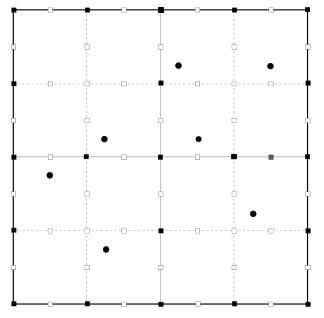
\includegraphics{portals.png}

\centering

\caption{Visualização dos portais em uma dissecção. Os quadrados de fundo preto representam portais para os níveis 1 e 2 da dissecção. Os quadrados de fundo branco representam portais para o nível 2 apenas. Fonte: \cite{Williamson}}
\label{fig:etspportais}
\end{figure}

Consideraremos rotas que entram e saem de cada quadrado somente por estes portais e chamaremos estas de \textit{$p$-rotas}. Dizemos que uma $p-$rota é \textit{$r-$light} se ela cruza, para cada subquadrado da dissecção, apenas $r$ vezes cada um de seus lados. 

A partir do lema e das notações que definimos, podemos apresentar dois teoremas que estamos estudando suas demonstrações e ainda não os provamos.

\begin{teorema}
Se escolhermos inteiros $(a,b)$ no intervalo $( -L' / 2,0]$ uniformemente e aleatoriamente, então com probabilidade de $1/2$ a dissecção $(a,b)$ tem uma $p$-rota $r-light$ de custo no máximo $(1 + \epsilon) OPT$ para um parâmetro de portais $ m = O\left( \frac{1}{\epsilon} \log L' \right) $ e $r = 2m + 4$
\end{teorema}

e 

\begin{teorema}
Se escolhermos inteiros $(a,b)$ no intervalo $( -L' / 2,0]$ uniformemente e aleatoriamente, então com probabilidade de $1/2$ a dissecção $(a,b)$ tem uma $p$-rota $r-light$ de custo no máximo $(1 + \epsilon) OPT$ para um parâmetro de portais $ m = O\left( \frac{1}{\epsilon} \log L' \right) $ e $r = O\left( \frac{1}{\epsilon} \right)$
\end{teorema}

Estes teoremas diferem quanto ao parâmetro $r$. Os passos necessários para concluí-los são: Demonstrar que é possível encontrar a menor $p$-rota por programação dinâmica em tempo polinomial e que é possível obter um esquema de aproximação polinomial se arbitrarmos a origem do quadrado $L'$ com a $(a,b)$-dissecção.

Deixaremos estes como tarefa pendente até o final de julho no cronograma desta proposta de qualificação.

\section{Considerações sobre o capítulo}

Vimos neste capítulo quatro problemas que possuem PTAS conhecido e usam programação dinâmica: Problema da mochila, escalonamento de tarefas em máquinas paralelas idênticas, empacotamento e caixeiro viajante euclidiano. As demonstrações foram baseadas no livro de Williamsom \cite{Williamson}.

Citamos aqui os autores de cada um dos algoritmos que estudamos. Para o problema da mochila, o algoritmo \ref{alg:pdmochila} foi apresentado por Lawler \cite{lawler}. O esquema de aproximação do algoritmo \ref{alg:pdmochilaptas} foi demonstrado por Ibarra e Kim \cite{ibarra}.

O esquema de aproximação para o escalonamento de tarefas com número constante de máquinas foi demonstrado por Graham \cite{graham}. Para o caso onde o número de máquinas faz parte da entrada do problema a demonstração foi realizada por Hochbaum e Shmoys \cite{hochbaum}. 

O esquema de aproximação para o problema do empacotamento foi demonstrado por Fernandez de la Vega e Lueker \cite{vega}.

O PTAS para o problema do caixeiro viajante foi proposto por Arora \cite{arora1998polynomial}. Não terminamos a demonstração deste problema, deixando-o como tarefa futura.

